\chapter{An Operational Semantics for the Essence of React Hooks}\label{chap:sem}
We now provide a formal operational semantics \Rtrace{} that is both high-level enough to abstract away React's implementation details, yet precise enough to reason about rendering behavior~(\cref{chap:rules}).
Up until now, we have implicitly discussed ``values'' using the syntax of \Rtrace, and we formally introduce semantic objects in~\cref{sec:dom}.
Then we describe the operational semantics of \Rtrace{} in~\cref{sec:sem}.

There are two layers that constitute the syntax and semantics of React Hooks:
\begin{description}
  \item[Base layer] describes standard computations within components.
    An excerpt from \cref{fig:syntax}:
    \begin{center}
      \begin{bnf}
        e : \dom{Exp} ::= () // true // false // $n$ // $x$  // $e \oplus e$ // $\print{e}$ // $\cond{e}{e}{e}$
          | $\seq{e}{e}$ // $\func{x}{e}$ // $\app{e}{e}$ // $\letbind{x}{e}{e}$ // $\dotsb$
      \end{bnf}
    \end{center}
  \item[Render layer] controls the rendering of components.
    An excerpt from \cref{fig:syntax}:
    \begin{center}
      \begin{bnf}[rccll]
        e : \dom{Exp} ::= $\dotsb$ // $C$ // $[\Overline{e}]$ // $\stbind{x}{e}{e}$ // $\eff{e}$
      \end{bnf}
    \end{center}
\end{description}

The base logic layer is crucial in order to build a rich UI with complex business logic.
For instance, Booleans and conditionals are required to write a toggleable button;
Functions and function applications are necessary to perform actions on behalf of user interaction.

Our choice of the base layer is not the only possible one.
We have chosen a minimal combination of features that can support the essence of Hooks---we can extend our base with strings, objects, recursive functions, etc.
Here, we will not burden ourselves with a layer not too relevant to the render logic.
In fact, all these features are included in our implementation of \Rtrace~(\cref{chap:impl}).

The render logic layer seems quite minimal, but we have seen its subtleties in~\cref{chap:over,chap:pit}.
We include all the base values to be used to represent views, and in addition, we include an array to model nested views and multiple children.
This is not a general purpose array---its elimination is when being used at the returning position of a component.
An example of an array view has been shown in the running examples in~\cref{chap:over}.
Each \reacttt{useState} Hook is (implicitly) labeled so that it is uniquely identified.
The returned value of \reacttt{useState} is a pair of current value~$x$ and the setter function~$x_{\texttt{set}}$.
\reacttt{useEffect} Hooks need not be labeled.

Note that we are only concerned with the timing aspects of the render semantics, not the visual layout; hence interactive UI elements such as a button is identified with its event handler.
As such, \reacttt{button f} is simply desugared into its event handler~\reacttt{f}.


\section{Semantic Objects}\label{sec:dom}
Semantic objects include base values~(\cref{subsec:base}) as well as the machinery that models the React runtime and Hooks~(\cref{subsec:machinery}).
The complete set of semantic objects is reproduced in~\cref{app:sec:dom} for reference.

\subsection{Base Values}\label{subsec:base}
The semantic objects for base values are formalized as follows:
\begin{center}
  \begin{minipage}{0.4791\textwidth}
    \begin{center}
      \begin{bnf}[rccll]
        v : $\dom{Val}$ ::= $k$ // $cl$ // $\dotsb$ :
        ;;
        k : $\dom{Const}$ ::= $\<\>$ // $\TT$ // $\FF$ // $n$ :
        ;;
        n :in: $\mathbb{Z}$
      \end{bnf}
    \end{center}
  \end{minipage}%
  \begin{minipage}{0.4791\textwidth}
    \begin{center}
      \begin{bnf}[rccll]
        cl : $\dom{Clos}$ ::= $\clos{x}{e}{\sigma}$ :
        ;;
        \sigma : $\dom{Env}$ ::= $[\Overline{x \mapsto v}]$ :
        ;;
        \omega : $\dom{Buffer}$ ::= $[\Overline{v}]$
      \end{bnf}
    \end{center}
  \end{minipage}
\end{center}
Base values are standard---constants~$k$ include the unit value~$\<\>$, Booleans~$\TT$ and~$\FF$, and integers~$n$.
To model the base layer using big-step semantics \citep{Kah87Natural} in~\cref{subsec:body}, bound variables are recorded in an environment~$\sigma = [\Overline{x \mapsto v}]$. %, an ordered list containing pairs of identifiers and values.
A function evaluates into a closure~$cl = \clos{x}{e}{\sigma}$. %, which is a pair of a function and an environment.
A buffer~$\omega = [\Overline{v}]$ holds a list of printed values.


\subsection{React Machinery}\label{subsec:machinery}
\paragraph{Extended Values}
To model the React machinery, we extend base values~$\dom{Val}$:
% WARNING: Unwrap the contents outside of the minipage when not needed, as well as the above/blowdisplayskip glues
% \vspace{\abovedisplayskip}
% \begin{minipage}{\linewidth} % To prevent pagebreak before the center env
  % \vspace{\abovedisplayskip}
  \begin{center}
    \begin{minipage}{0.4791\textwidth}
      \begin{center}
        \begin{bnf}[rccll]
          v : $\dom{Val}$ ::=  $\dotsb$ // $C$  // $cs$ // $[\Overline{s}]$ // $\<\ell, p\>$ :
          ;;
          cs : $\dom{ComSpec}$ ::= $\<C, v\>$ :
          ;;
          s : $\dom{ViewSpec}$ ::= $k$ // $cl$ // $cs$ // $[\Overline{s}]$ :
        \end{bnf}
      \end{center}
    \end{minipage}%
    \begin{minipage}{0.4791\textwidth}
      \begin{center}
        \begin{bnf}[rccll]
          \delta : $\dom{DefTable}$ ::= $[\Overline[\ell]{C \mapsto \deftabent{x}{e}}]$ :
          ;;
          \ell :in: $\mathbb{N}$ :
          ;;
          p :in: $\dom{Path} = \mathbb{N}$ :
        \end{bnf}
      \end{center}
    \end{minipage}
  \end{center}
%   \vspace{\belowdisplayskip}
% \end{minipage}
A component name~$C$ is a value as-is.
All component names are determined statically and their definitions are looked up using a \emph{definition table~$\delta = [\Overline[\ell]{C \mapsto \deftabent{x}{e}}]$}.
Thus (mutually) recursive components are permitted in \Rtrace, and we do not model legacy higher-order components \cite{Met25Higher}.
A \emph{view spec} is either a constant value~$k$, a closure~$cl$, a component spec~$cs$, or an array view spec~$[\Overline{s}]$.
A constant and a closure view spec represent leaf views, whereas a component and an array view spec represent composite views.
A constant view spec is simply realized into a view that shows its string representation.
A closure view spec, when realized into a view, represents an event handler---this models UI elements such as a button, an input field, a checkbox, etc.
A component spec~$cs = \<C, v\>$ is simply a pair of a component name and its argument.
This represents a specification of a view that may be realized into a view hierarchy.
An array view spec~$[\Overline{s}]$ is an array of view specs~$s$, representing structured child views.

A setter closure~$\<\ell, p\>$, which is the semantic value of a setter function, is a pair of a label~$\ell$ from the originating \reacttt{useState} Hook and a \emph{path}~$p$ to the corresponding view in the view tree.
A path~$p$ is a unique natural number used to identify each view in the view tree.
We shall take a look at the view tree structure~$m$ in a moment.

\paragraph{Tree Memory}
We introduce \emph{tree memory}~$m$ to model the view hierarchy:
\begin{center}
  \begin{bnf}[rccll]
    m : $\dom{TreeMem}$ ::= $[\Overline{p \mapsto \pi}]$ :
    ;;
    \pi : $\dom{View}$ ::= $\view{cs}{\{\Overline{d}\}}{\rho}{q}{t}$ :
    ;;
    d : $\dom{Decision}$ ::= \dec{Check} // \dec{Effect} :
  \end{bnf}
  \vspace*{-0.2\baselineskip}
  \begin{center}
    \begin{minipage}{0.4791\textwidth}
      \begin{center}
        \begin{bnf}[rccll]
          t : $\dom{Tree}$ ::= $k$ // $cl$ // $p$ // $[\Overline{t}]$ :
          ;;
          \rho : $\dom{SttStore}$ ::= $[\Overline[\ell]{\ell \mapsto \sttstent{v}{q}}]$ :
        \end{bnf}
      \end{center}
    \end{minipage}%
    \begin{minipage}{0.4791\textwidth}
      \begin{center}
        \begin{bnf}[rccll]
          q : $\dom{JobQ}$ ::= $[\Overline[\ell]{cl}]$ :
          ;;
          \Sigma : $\dom{Context}$ ::= $m$ // $\pi$ :
        \end{bnf}
      \end{center}
    \end{minipage}
  \end{center}
\end{center}
The entire view hierarchy is stored in a tree memory~$m$ which maps each path~$p$ to a view~$\pi$.
A view is a realized component that is mounted or to-be-mounted into a tree memory.
Each mounted view~$\pi$ is assigned a unique path~$p$ where $p$~is a valid path of a tree memory~$m$, i.e., $p \in \domain m$.
It consists of a component spec~$cs$, a decision~$d$, an effect queue~$q$, and a child tree~$t$.
When a component body is evaluated, the runtime keeps track of its decision set---\dec{Check} for checking the component for retry or re-render, and \dec{Effect} for running Effects after this render.
Decisions \dec{Check} and \dec{Effect} have been explained informally in~\cref{subsec:infloop,subsec:topset}, and all components first begin with an empty decision set.
A state store~$\rho$ for each view is used to store the current state value~$v$ and the queued updates~$q$ from setter function from the \reacttt{useState} Hook.
These are keyed using the corresponding label~$\ell$ of \reacttt{useState}.
An effect queue~$q$ is a queue of Effects from the \reacttt{useEffect} Hook.
A child~$t$ is either a terminal view~$k$, an event handler~$cl$, a path~$p$ to another view, or an array of children~$[\Overline{t}]$.
We also introduce a context~$\Sigma$, which can be either a tree memory~$m$ or a view~$\pi$.
This distinction exists because one evaluation rule (\Rule{AppSetNormal}) requires the whole tree memory~$m$, while the others only require the local view~$\pi$ in their context.
The whole-memory context is used to describe a component updating another, e.g., a button in a child component updating its parent's state.

\begin{figure}[t]
  \begin{center}
    \begin{minipage}{.27\textwidth}
      \begin{reactcode}
  let Bin n =
    if n = 0 then () else
    [Bin(n-1), Bin(n-1)];;
  Bin 2
      \end{reactcode}
    \end{minipage}%
    \begin{minipage}{.73\textwidth}
      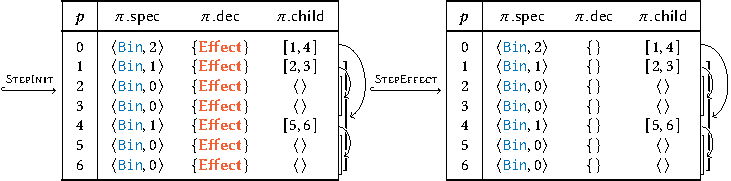
\includegraphics[width=\linewidth]{images/treemem.pdf}
    \end{minipage}
  \end{center}
  \caption{Visualization of a tree memory and render step transitions for a simple recursive component.}\label{fig:bin}
\end{figure}

To give a visual intuition of how tree memory represents view hierarchy, \cref{fig:bin} shows a tree memory for a simple recursive component~\reacttt{Bin} that creates a complete binary tree of height~2.
The root tree is assigned path~$p = 0$, and each subtree receives a unique path in the order of initialization (\cref{fig:init},~\cref{subsec:body}).
The view hierarchy can be reconstructed by traversing the \field{child} field of each view in the tree memory.
The render step transitions \Rule{StepInit} and \Rule{StepEffect} along with the decisions shown in \cref{fig:bin} are explained in detail in~\cref{subsec:lifecycle}.


\paragraph{Phase}
While evaluating an expression, we maintain a phase~$\phi$:
\begin{center}
  \begin{bnf}[rccll]
    \phi : $\dom{Phase}$ ::= \phase{Init} // \phase{Succ} // \phase{Normal} :
  \end{bnf}
\end{center}
\phase{Init}\footnote{We use \phase{blue sans-serif} to emphasize a phase.} phase is used when evaluating a component for the first time to be mounted into a tree memory.
At this phase, all states are evaluated from the initial expressions of \reacttt{useState}s.
Successive calls to a component function are done in \phase{Succ} phase, where states are retrieved from a state store.
The main expression, Effects, and event handlers are evaluated in \phase{Normal} phase.


\paragraph{Mode}
We model each (re-)render as a transition of global states, and we introduce a mode~$\mu$ to keep track of the state of the \Rtrace{} engine:
\begin{center}
  \begin{bnf}[rccll]
    \mu : $\dom{Mode}$ ::= $\rendermode$ \textrm{(rendered)} // $\checkmode$ \textrm{(check)} // $\eloopmode$ \textrm{(event loop)} :
  \end{bnf}
\end{center}
Rendered mode~$\rendermode$ represents a state where the UI has been rendered on the screen and is waiting for the queued Effects to run.
Check mode~$\checkmode$ represents a state where the runtime will check for a re-render.
When a re-render is not required, we enter event loop mode~$\eloopmode$ and wait for an input.


\section{Operational Semantics}\label{sec:sem}
All semantic functions\footnote{Semantic functions are typeset using an \sem{italicized sans-serif} font.} and evaluation relations, along with their dependencies and required contexts, are summarized in \cref{fig:dependencies}.
\begin{figure}[t]
  \centering
  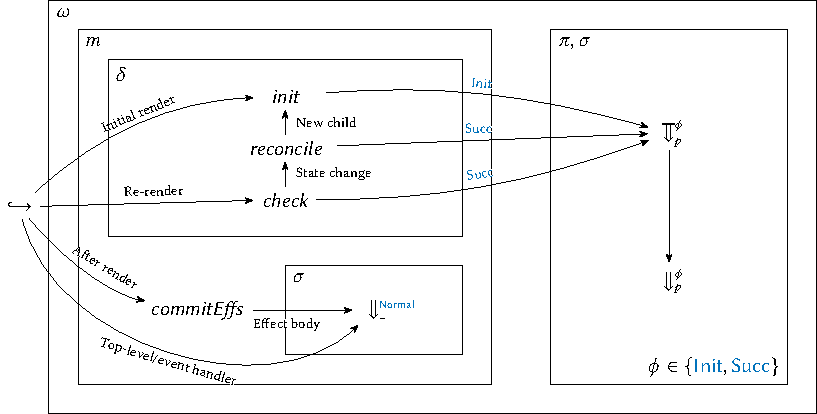
\includegraphics[width=.85\textwidth]{images/diagram.pdf}
  \caption{Semantic function dependencies.}\label{fig:dependencies}
\end{figure}
We give a brief overview of the semantic functions and relations before we formally introduce them in~\cref{subsec:body,subsec:commiteffs,subsec:reconciliation}:
\begin{itemize}
  \item $\<e, \delta\> \text{ or }\<t, m, \omega, \delta, \mu\> \smallstep \<t, m', \omega', \delta, \mu'\>$ is a render step transition (\cref{fig:step}).
    Read this as ``Initially, under definition table~$\delta$, main expression~$e$ transitions to root tree~$t$, tree memory~$m'$, and output buffer~$\omega'$, entering mode~$\mu'$,'' or ``Given root tree~$t$ under definition table~$\delta$, tree memory~$m$ and output buffer~$\omega$ in mode~$\mu$ transition to~$m'$ and $\omega'$, entering mode~$\mu'$.''

  \item $\Step<\phi><p>[\Sigma, \sigma]{e}{v, \Sigma', \omega}$ is an evaluation of an expression (\cref{fig:eval}).
    Read this as ``In phase~$\phi$ at path~$p$, expression~$e$ under environment~$\sigma$ and context~$\Sigma$ evaluates to value~$v$, producing a modified context~$\Sigma'$ and output~$\omega$.''

  \item $\Step*<\phi><p>[\pi, \sigma]{e}{s, \pi', \omega}$ is a possibly retrying evaluation of a component body until it becomes idle (\cref{fig:evalmult}).
    Read this as ``In phase~$\phi$ at path~$p$, component body~$e$ of view~$\pi$ under environment~$\sigma$ eventually evaluates to view spec~$s$, producing a modified view~$\pi'$ and output~$\omega$.''

  \item $m, \delta \vdash \sem{init}(s) = \<t, m', \omega\>$ is a rendering of a view spec in an initial render (\cref{fig:init}).
    Read this as ``Under definition table~$\delta$, view spec~$s$ initially renders into tree~$t$, modifying tree memory from~$m$ to~$m'$ and printing~$\omega$.''

  \item $m \vdash \sem{commitEffs}(t) = \<m', \omega\>$ is committing queued Effects (\cref{fig:commiteffs}).
    Read this as ``Committing Effects of tree~$t$ modifies tree memory from~$m$ to~$m'$ and prints~$\omega$.''

  \item $m, \delta \vdash \sem{check}(t) = \<\mu, m', \omega\>$ is checking and updating a tree for a re-render (\cref{fig:check}).
    Read this as ``Under definition table~$\delta$, tree~$t$ re-renders with modified tree memory~$m'$ from~$m$ and prints~$\omega$'' when~$\mu = \rendermode$, and ``Under definition table~$\delta$, tree~$t$ does not re-render but modifies tree memory from~$m$ to~$m'$ and prints~$\omega$'' when~$\mu = \eloopmode$; $\mu$ cannot be $\checkmode$.

  \item $m, \delta \vdash \sem{reconcile}(t, s) = \<t', m', \omega\>$ is reconciling a tree with a possibly updated view spec (\cref{fig:reconcile}).
    Read this as ``Under definition table~$\delta$, tree~$t$ is reconciled as~$t'$ with respect to view spec~$s$, modifying tree memory from~$m$ to~$m'$ and printing~$\omega$.''
\end{itemize}

\begin{nota}
We explain notation used in the evaluation rules.
When a rule has premises~$J_i$ for~$l \le i \le u$, we write~$(J_i)_{i = l}^u$.
We use~$\concat$ for list concatenation, e.g., $x \concat x'$, and~$\Concat_{i=l}^u x_i$ for concatenating~$x_l, \dotsc, x_u$.
For bindings~$X$, $X[x \mapsto v]$ updates~$X$ with~$x \mapsto v$, and~$X[x]$ retrieves the value~$v$ when $X$~has a binding~$x \mapsto v$.
For a structure~$X$ with a field~\field{f}, $X\{\fv{f}{v}\}$ updates field~\field{f} to~$v$, and~$X.\field{f}$ accesses field~\field{f}.
We use meta-level let-bindings~``let $x = v$ in $\dotsc$'' inside meta-level structure or list updates when convenient.
Meta-level conditional~$\scond{b}{x}{y}$ chooses~$x$ when~$b$ holds and chooses~$y$ otherwise.
\end{nota}


\subsection{Render Loop}\label{subsec:lifecycle}
We model the React event loop with render step transitions in \cref{fig:step}.
\begin{figure}[t]
  \centering
  \hfill\fbox{$\<e, \delta\> \text{ or }\<t, m, \omega, \delta, \mu\> \smallstep \<t, m', \omega', \delta, \mu'\>$}
\begin{mathpar}
\inferrule[StepInit]{
  \Step<\phase{Normal}><->[[], []]{e}{s, [], \omega} \\
  [] \vdash \sem{init}(s) = \<t, m, \omega'\>
}{
  \<e, \delta\> \smallstep \<t, m, \omega \concat \omega', \delta, \rendermode\>
} \and
\inferrule[StepEffect]{
  m \vdash \sem{commitEffs}(t) = \<m', \omega'\>
}{
  \<t, m, \omega, \delta, \rendermode\> \smallstep \<t, m', \omega \concat \omega', \delta, \checkmode\>
} \and
\inferrule[StepCheck]{
  m, \delta \vdash \sem{check}(t) = \<\mu, m', \omega'\> \\
}{
  \<t, m, \omega, \delta, \checkmode\> \smallstep \<t, m', \omega \concat \omega', \delta, \mu\>
} \and
\inferrule[StepEvent]{
  \clos{x}{e}{\sigma} \in \sem{handlers}(m, t) \\
  \Step<\phase{Normal}><->[m, \sigma[x \mapsto \<\>]]{e}{v, m', \omega'} \\
}{
  \<t, m, \omega, \delta, \eloopmode\> \smallstep \<t, m', \omega \concat \omega', \delta, \checkmode\>
}
\end{mathpar}
  \caption{Render step transitions.}\label{fig:step}
\end{figure}

Given a program~$P$, the loop begins with an initial state~$\<e, \delta\>$, where $e$~is the main expression of~$P$ and $\delta$ is the definition table of all components defined in~$P$.
Note that the definition table~$\delta$ and the root tree~$t$ (once initialized) remain unchanged during transitions.

First, we evaluate the main expression~$e$ into a view spec~$s$ and initialize it into a tree~$t$ with an updated tree memory~$m$; we enter the rendered mode~$\rendermode$ (\Rule{StepInit}).
We call this a rendered mode because the root tree~$t$ and all of its descendants as described in~$m$ have been \emph{rendered on screen.}
Then we commit all the queued Effects of~$t$ and its descendants, after which we enter the check mode~$\checkmode$ (\Rule{StepEffect}).
In check mode~$\checkmode$, we check for any state update under~$t$.
If there is an update, we render again and enter the rendered mode~$\rendermode$; otherwise, we enter the event loop mode~$\eloopmode$ (\Rule{StepCheck}).
In event loop mode~$\eloopmode$, we wait for user input to be handled by an event handler.
If input occurs, we evaluate the corresponding handler body, which then requires a state update check (\Rule{StepEvent}).

Returning to the simple example shown in \cref{fig:bin}, all the views in the tree memory contain \dec{Effect} decisions after the \Rule{StepInit} transition, as they are freshly mounted and React needs to check for any defined Effects (of which there are none in the example).
All the \dec{Effect} decisions are then cleared after the \Rule{StepEffect} transition.
No state updates have been made---there are no \dec{Check} decisions---and \Rule{StepCheck} transitions to the same tree memory, this time in event loop mode~$\eloopmode$.

To elaborate on how the transition \Rule{StepInit} evaluates the main expression and initializes the evaluated view spec, we turn our attention to the evaluation rules for expressions~(\cref{subsec:eval}) and the initialization rules (\cref{subsec:body}).


\subsection{Evaluating an Expression}\label{subsec:eval}
\paragraph{Single Evaluation}
We present how an expression is evaluated in a big-step semantics in \cref{fig:eval}.
The rules relevant to the render logic are included here, which includes \reacttt{useState} and the \reacttt{useEffect} Hooks, component application, and state updates.
Standard rules related to the base logic are not presented---\Rule{AppFunc} and \Rule{Print} are included for clarity.
The complete operational semantics of expressions is available in~\cref{app:sec:sem}.
\begin{figure}[t]
  \centering
  \hfill\fbox{$\Step<\phi><p>[\Sigma, \sigma]{e}{v, \Sigma', \omega}$}
  \begin{mathpar}
    \inferrule[AppFunc]{
  \Step{e_1}{\clos{x}{e}{\sigma'}, \Sigma_1, \omega_1} \\
  \Step[\Sigma_1, \sigma]{e_2}{v_2, \Sigma_2, \omega_2} \\
  \Step[\Sigma_2, \sigma'[x \mapsto v_2]]{e}{v', \Sigma', \omega'}
}{
  \Step{\app{e_1}{e_2}}{v', \Sigma', \omega_1 \concat \omega_2 \concat \omega'}
} \and
\inferrule[AppCom]{
  \Step{e_1}{C, \Sigma_1, \omega_1} \\
  \Step[\Sigma_1, \sigma]{e_2}{v, \Sigma_2, \omega_2}
}{
  \Step{\app{e_1}{e_2}}{\<C, v\>, \Sigma_2, \omega_1 \concat \omega_2}
} \and
\inferrule[AppSetComp]{
  \Step[\pi, \sigma]{e_1}{\<\ell, p\>, \pi_1, \omega_1} \\
  \Step[\pi_1, \sigma]{e_2}{cl, \pi_2, \omega_2} \\
  \phi \in \{\phase{Init}, \phase{Succ}\}
}{
  \Step[\pi, \sigma]{\app{e_1}{e_2}}{
    \<\>,
    \pi_2\!\left\{
      \begin{spreadlines}{0pt}
        \begin{lgathered}
          \text{let $\rho = \pi_2.\field{sttst},\ vq = \rho[\ell]$ in} \\
          \begin{aligned}
            \field{dec} &\colon \pi_2.\field{dec} \cup \{\dec{Check}\} \\
            \field{sttst} &\colon \rho[\ell \mapsto vq\{\fv{sttq}{vq.\field{sttq} \concat [cl]}\}]
          \end{aligned}
        \end{lgathered}
      \end{spreadlines}
    \right\},
    \omega_1 \concat \omega_2
  }
} \and
\inferrule[AppSetNormal]{
  \Step<\phase{Normal}><->[m, \sigma]{e_1}{\<\ell, p\>, m_1, \omega_1} \\
  \Step<\phase{Normal}><->[m_1, \sigma]{e_2}{cl, m_2, \omega_2} \\
}{
  \Step<\phase{Normal}><->[m, \sigma]{\app{e_1}{e_2}}{
    \<\>,
    m_2\!\left[
      \begin{spreadlines}{0pt}
        \begin{lgathered}
          \text{let $\pi = m_2[p],\ \rho = \pi.\field{sttst},\ vq = \rho[\ell]$ in} \\
          p \mapsto \pi\!\left\{
            \begin{aligned}
              \field{dec} &\colon \pi.\field{dec} \cup \{\dec{Check}\} \\
              \field{sttst} &\colon \rho[\ell \mapsto vq\{\fv{sttq}{vq.\field{sttq} \concat [cl]}\}]
            \end{aligned}
          \right\}
        \end{lgathered}
      \end{spreadlines}
    \right],
    \omega_1 \concat \omega_2
  }
} \and
\inferrule[SttBind]{
  \Step<\phase{Init}>[\pi, \sigma]{e_1}{v_1, \pi_1, \omega_1} \\
  \Step<\phase{Init}>[{
    \begin{spreadlines}{0pt}
      \pi_1\!\left\{
        \fv{sttst}{
          \pi_1.\field{sttst}\!\left[\ell \mapsto \sttstent*{v_1}{[]}\right]
        }
      \right\}\!,
      \sigma\!\left[
        \begin{aligned}
          x &\mapsto v_1 \\
          x_{\textsf{set}} &\mapsto \<\ell, p\>
        \end{aligned}
      \right]
    \end{spreadlines}
  }]{e_2}{v_2, \pi_2, \omega_2}
}{
  \Step<\phase{Init}>[\pi, \sigma]{\stbind[\ell]{x}{e_1}{e_2}}{v_2, \pi_2, \omega_1 \concat \omega_2}
} \and
\inferrule[SttReBind]{
  \pi_0.\field{sttst}[\ell] = \bigl\{
    \fv{val}{v_0},\:\fv{sttq}{[\Overline{\clos{x_i}{e'_i}{\sigma_i}}]_{i = 1}^n}
  \bigr\} \\
  \bigl(\Step[\pi_{i-1}, \sigma_i[x_i \mapsto v_{i-1}]]{e'_i}{v_i, \pi_i, \omega_i}\bigr)_{i = 1}^n \\
  \Step[{
    \begin{spreadlines}{0pt}
      \pi_n\!\left\{
        \begin{aligned}
          \field{dec} &\colon \pi_n.\field{dec} \cup \scond{v_n \not\equiv v_0 }{\{\dec{Effect}\}}{\emptyset} \\
          \field{sttst} &\colon \pi_n.\field{sttst}[\ell \mapsto \sttstent{v_n}{[]}]
        \end{aligned}
      \right\}\!,
      \sigma\!\left[
        \begin{aligned}
          x &\mapsto v_n \\
          x_{\textsf{set}} &\mapsto \<\ell, p\>
        \end{aligned}
      \right]
    \end{spreadlines}
  }]{e_2}{v, \pi', \omega'}
}{
  \Step<\phase{Succ}>[\pi_0, \sigma]{\stbind{x}{e_1}{e_2}}{v, \pi', ({\textstyle\Concat_{i = 0}^n \omega_i}) \concat \omega'}
} \and
\inferrule[Eff]{
  \phi \in \{\phase{Init}, \phase{Succ}\}
}{
  \Step[\pi, \sigma]{\eff{e}}{
    \begin{spreadlines}{0pt}
      \<\>,
      \pi\{ \fv{effq}{\pi.\field{effq} \concat [\clos{\_}{e}{\sigma}]} \},
      []
    \end{spreadlines}
  }
} \and
\inferrule[Print]{
  \Step{e}{v, \Sigma', \omega}
}{
  \Step{\print{e}}{\<\>, \Sigma', \omega \concat [v]}
}
  \end{mathpar}
  \caption{Evaluation of an expression (an excerpt).}\label{fig:eval}
\end{figure}

An environment~$\sigma$, context~$\Sigma$, phase~$\phi$, and path~$p$ are required for evaluating an expression~$e$.
A path is not available (written as $-$ in \cref{fig:eval}) in the \phase{Normal} phase.
Evaluation rules that are only applicable in the context of a component body evaluation (\Rule{AppSetComp}, \Rule{SttBind}, \Rule{SttReBind}, and \Rule{Eff}), i.e., in the \phase{Init} and \phase{Succ} phase, require the context~$\Sigma$ to be a view~$\pi$.
A noteworthy case is \Rule{AppSetNormal}, the only rule applicable in the \phase{Normal} phase only.
All other rules permit both~$\pi$ and~$m$ as a context~$\Sigma$.
The output buffer~$\omega$ stores the printed values sequentially (\Rule{Print}).

It is important to note that component definitions are not required during evaluation of an expression.
Hence, a component application is nothing more than packing the evaluated component name~$C$ and the argument~$v$ in a pair (\Rule{AppCom}).
The actual function bound to the component name is neither invoked nor required at this point.

The \reacttt{useState} Hook behaves differently in the \phase{Init} and \phase{Succ} phases.
In the \phase{Init} phase, the initial value~$v_1$ is evaluated from the argument~$e_1$, which is then stored in the view's state store \field{sttst} at label~$\ell$ of \reacttt{useState}, along with an empty state update queue \field{sttq} (\Rule{SttBind}).
In addition, the state variable~$x$ and the setter function~$x_{\texttt{set}}$ are bound to the initial value~$v_1$ and the setter closure, which is a pair~$\<\ell, p\>$, so that the value of the state can be read and set.

In the \phase{Succ} phase, all the queued updates in \field{sttq} are processed while evaluating the corresponding \reacttt{useState} Hook (\Rule{SttReBind}).
After evaluating all the updates, we compare the final state value~$v_n$ with the initial value~$v_0$.
If they are equivalent ($v_n \equiv v_0$), we simply keep the previous decision \field{dec}.
Otherwise ($v_n \nequiv v_0$), the component adds the \dec{Effect} decision to its decision so that it runs its Effects after rendering.
The state update queue \field{sttq} is flushed and the state variable and the setter function are bound appropriately.

State updates via setter function applications behave differently when evaluating a component ($\phi \in \{\phase{Init}, \phase{Succ}\}$) compared to when evaluating Effects or event handlers ($\phi = \phase{Normal}$).
During component body evaluation, calling a setter function of another component is not allowed, hence the path~$p$ in the setter closure must match with the context (\Rule{AppSetComp}).
The official React runtime logs an error message when a component evaluation invokes a setter function of another component.
Setting the component's state during the evaluation of its body adds the \dec{Check} decision and queues the provided update closure~$cl$.
The \dec{Check} decision triggers a re-evaluation of the component---this behavior is formalized in \cref{fig:evalmult}.

State updates in the \phase{Normal} phase lift the restriction of ``inter-component'' updates.
The setter closure~$\<\ell, p\>$ is used to queue the update closure~$cl$ in the correct tree at path~$p$ and the correct label~$\ell$ in the state queue \field{sttq} (\Rule{AppSetNormal}).
The \dec{Check} decision is added to the view's decision, to mark that a state update has been queued.
The marked views are later processed in batches~(\cref{subsec:reconciliation}).

\paragraph{Retrying Evaluation}
The evaluation of a component body starts with a \emph{retrying evaluation}, where the body is repeatedly evaluated until the \(\dec{Check}\) decision is no longer present.
Before each evaluation, the Effect queue is cleared so that Effects are re-collected during execution.
The rationale is that re-evaluated view specs are discarded except for the last one, and Effects associated with the discarded view specs must also be discarded.
In addition, the \(\dec{Check}\) decision is removed beforehand to determine whether the evaluation triggers another \(\dec{Check}\).
The component body is then evaluated, and evaluation stops when \(\dec{Check}\) is no longer present (\Rule{EvalOnce}).
If the evaluation results in another \(\dec{Check}\) decision, re-evaluation is performed in the \phase{Succ} phase (\Rule{EvalMult}).

\begin{figure}[t]
  \centering
  \hfill\fbox{$\Step*<\phi><p>[\pi, \sigma]{e}{s, \pi', \omega}$}
\begin{mathparpagebreakable}
  \inferrule[EvalOnce]{
    \Step[\pi\{\fv{dec}{\pi.\field{dec}\setminus\{\dec{Check}\}},\fv{effq}{[]}\}, \sigma]{e}{s, \pi', \omega} \\
    \dec{Check} \notin \pi'.\field{dec} \\
    \phi \in \{\phase{Init}, \phase{Succ}\}
  }{
    \Step*[\pi, \sigma]{e}{s, \pi', \omega}
  } \and
  \inferrule[EvalMult]{
    \Step[\pi\{\fv{dec}{\pi.\field{dec}\setminus\{\dec{Check}\}},\fv{effq}{[]}\}, \sigma]{e}{s, \pi', \omega} \\
    \dec{Check} \in \pi'.\field{dec} \\
    \Step*<\phase{Succ}>[\pi', \sigma]{e}{s', \pi'', \omega'} \\
    \phi \in \{\phase{Init}, \phase{Succ}\}
  }{
    \Step*[\pi, \sigma]{e}{s', \pi'', \omega \concat \omega'}
  }
\end{mathparpagebreakable}
  \caption{Retrying evaluation of a component body.}\label{fig:evalmult}
\end{figure}

Note that a component may indefinitely decide to \dec{Check}, which will lead to an infinite retrial issue described in \cref{subsec:topset}.
React runtime raises an exception after 25~retrials.


\subsection{Initial Render}\label{subsec:body}
When a view is initially rendered, it is initialized from a view spec (\cref{fig:init}).
A constant (\Rule{InitConst}), closure (\Rule{InitClos}), and array view spec initialization (\Rule{InitArray}) are straightforward.
\begin{figure}[t]
  \centering
  \hfill\fbox{$m, \delta \vdash \sem{init}(s) = \<t, m', \omega\>$}
\begin{mathparpagebreakable}
  \inferrule[InitConst]{ }{m, \delta \vdash \sem{init}(k) = \<k, m, []\>} \and
  \inferrule[InitClos]{ }{m, \delta \vdash \sem{init}(cl) = \<cl, m, []\>} \and
  \inferrule[InitArray]{
    \bigl(m_{i-1}, \delta \vdash \sem{init}(s_i) = \<t_i, m_i, \omega_i\>\bigr)_{i = 1}^n
  }{
    m_0, \delta \vdash \sem{init}([\Overline{s_i}]_{i = 1}^n) = \<[\Overline{t_i}]_{i = 1}^n, m_n, {\textstyle\Concat_{i = 1}^n \omega_i}\>
  } \and
  \inferrule[InitCom]{
    m \vdash p\:\judge{fresh} \\
    \delta[C] = \deftabent{x}{e} \\
    \Step*<\phase{Init}>[
      \view{\<C, v\>}{\emptyset}{[]}{[]}{\<\>},
      [x \mapsto v]
    ]{e}{s, \pi, \omega} \\
    m[p \mapsto \pi], \delta \vdash \sem{init}(s) = \<t, m', \omega'\>
  }{
    m, \delta \vdash \sem{init}(\<C, v\>) = \bigl\<p, m'[p \mapsto \pi\{\fv{dec}{\{\dec{Effect}\}}, \fv{child}{t}\}], \omega \concat \omega'\bigr\>
  }
\end{mathparpagebreakable}
  \caption{Initialization of a view spec.}\label{fig:init}
\end{figure}

To initialize a component spec~$\<C, v\>$, a fresh path~$p$ with respect to the tree memory~$m$ is generated, and the definition table~$\delta$ is used to look up the component definition for name~$C$ (\Rule{InitCom}).
First, an empty view with the component spec, an empty decision set, and a (placeholder)~unit child is created.
This view is used as a context to evaluate the component body in the \phase{Init} phase with the parameter~$x$ bound to~$v$, which produces a view spec~$s$ and an updated view~$\pi$.
After mounting the updated~$\pi$ at path~$p$ in tree memory~$m$, view spec~$s$ is recursively initialized to get the child tree~$t$.
Finally, the \dec{Effect} decision is added to the view to ensure the queued Effects are run after the initial render, and the \field{child} field is set to~$t$.
Note that the initialization of the child tree does not modify the parent view~$\pi$.

\subsection{Committing Effects After Render}\label{subsec:commiteffs}
After a view has been rendered, the queued Effects must be executed.
The rules in \cref{fig:commiteffs} describe this process.
For a constant (\Rule{CommitEffsConst}) and a closure (\Rule{CommitEffsClos}), there are no Effects to commit, so the tree memory remains unchanged.
For an array of trees (\Rule{CommitEffsArray}), we recursively commit the Effects of each child tree.
\begin{figure}[t]
  \centering
  \hfill\fbox{$m \vdash \sem{commitEffs}(t) = \<m', \omega\>$}
\begin{mathparpagebreakable}
  \inferrule[CommitEffsConst]{ }{m \vdash \sem{commitEffs}(k) = \<m, []\>} \and
  \inferrule[CommitEffsClos]{ }{m \vdash \sem{commitEffs}(cl) = \<m, []\>} \and
  \inferrule[CommitEffsArray]{
    \bigl(m_{i-1} \vdash \sem{commitEffs}(t_i) = m_i, \omega_i\bigr)_{i = 1}^n
  }{
    m_0 \vdash \sem{commitEffs}([\Overline{t_i}]_{i = 1}^n) = \<m_n, {\textstyle\Concat_{i = 1}^n \omega_i}\>
  } \and
  \inferrule[CommitEffsPathIdle]{
    \dec{Effect} \notin m[p].\field{dec} \\
    m \vdash \sem{commitEffs}(m[p].\field{child}) = \<m', \omega\> \\
  }{
    m \vdash \sem{commitEffs}(p) = \<m', \omega\>
  } \and
  \inferrule[CommitEffsPath]{
    \dec{Effect} \in m[p].\field{dec} \\
    m[p].\field{effq} = [\Overline{\clos{\_}{e_i}{\sigma_i}}]_{i = 1}^n \\
    m \vdash \sem{commitEffs}(m[p].\field{child}) = \<m_0, \omega_0\> \\
    \bigl(
      \Step<\phase{Normal}><->[m_{i-1}, \sigma_i]{e_i}{v_i, m_i, \omega_i}
    \bigr)_{i = 1}^n
  }{
    m \vdash \sem{commitEffs}(p) = \bigl\<m_n\bigl[p \mapsto m_n[p]\{\fv{dec}{m_n[p].\field{dec} \setminus \{\dec{Effect}\}}\}\bigr], {\textstyle\Concat_{i = 0}^n \omega_i}\bigr\>
  }
\end{mathparpagebreakable}
  \caption{Committing Effects.}\label{fig:commiteffs}
\end{figure}

For a path to a view, Effects are committed only when the view has decided to.
If the view has not decided to commit \dec{Effect}s, only the Effects of its child are executed, and the view's Effects are skipped (\Rule{CommitEffsPathIdle}).
If the view's decision includes \dec{Effect}, the Effects of its child are committed first, and then the view's Effects are executed in order (\Rule{CommitEffsPath}).
Each Effect is evaluated in the \phase{Normal} phase, allowing it to update any component's states in the tree.

Effects execution follows a post-order traversal---the child's Effects are executed first, followed by those of its parent.
Additionally, Effects are executed following their original syntactic order.


\subsection{Checking, Re-Render, and Reconciliation}\label{subsec:reconciliation}
\paragraph{Checking for Re-Render}
In check mode~$\checkmode$, which is after committing Effects or handling an event, the runtime checks and re-renders a tree if needed.
This is carried out with semantic function~\sem{check} shown in \cref{fig:check}.
When a tree or any of its descendants requires a re-render, \sem{check} performs the re-render and returns either of~$\rendermode$ or~$\eloopmode$.
It also returns the modified tree memory.
\begin{figure}[t]
  \centering
  \hfill\fbox{$m, \delta \vdash \sem{check}(t) = \<\mu, m', \omega\>$}
\begin{mathparpagebreakable}
  \inferrule[CheckConst]{ }{m, \delta \vdash \sem{check}(k) = \<\eloopmode, m, []\>} \and
  \inferrule[CheckClos]{ }{m, \delta \vdash \sem{check}(cl) = \<\eloopmode, m, []\>} \and
  \inferrule[CheckArray]{
    \bigl(m_{i-1}, \delta \vdash \sem{check}(t_i) = \<\mu_i, m_i, \omega_i\>\bigr)_{i = 1}^n
  }{\textstyle
    m_0, \delta \vdash \sem{check}([\Overline{t_i}]_{i = 1}^n) = \<\bigsqcup_{i = 1}^n \mu_i, m_n, {\textstyle\Concat_{i = 1}^n \omega_i}\>
  } \and
  \inferrule[CheckIdle]{
    m[p] = \pi \\
    \dec{Check} \notin \pi.\field{dec} \\
    m, \delta \vdash \sem{check}(\pi.\field{child}) = \<\mu, m', \omega\>
  }{\textstyle
    m, \delta \vdash \sem{check}(p) = \<\mu, m', \omega\>
  } \and
  \inferrule[CheckNoEffect]{
    m[p] = \pi \\
    \dec{Check} \in \pi.\field{dec} \\
    \pi.\field{spec} = \<C, v\> \\
    \delta[C] = \deftabent{x}{e} \\
    \Step*<\phase{Succ}>[
      \pi,
      [x \mapsto v]
    ]{e}{\_, \pi', \omega} \\
    \dec{Effect} \notin \pi'.\field{dec} \\
    m, \delta \vdash \sem{check}(\pi.\field{child}) = \<\mu, m', \omega'\>
  }{\textstyle
    m, \delta \vdash \sem{check}(p) = \<\mu, m'[p \mapsto \pi'], \omega \concat \omega'\>
  } \and
  \inferrule[CheckEffect]{
    m[p] = \pi \\
    \dec{Check} \in \pi.\field{dec} \\
    \pi.\field{spec} = \<C, v\> \\
    \delta[C] = \deftabent{x}{e} \\
    \Step*<\phase{Succ}>[
      \pi,
      [x \mapsto v]
    ]{e}{s, \pi', \omega} \\
    \dec{Effect} \in \pi'.\field{dec} \\
    m, \delta \vdash \sem{reconcile}(\pi.\field{child}, s) = \<t', m', \omega'\> \\
  }{\textstyle
    m, \delta \vdash \sem{check}(p) = \<\rendermode, m'[p \mapsto \pi'\{\fv{child}{t'}\}], \omega \concat \omega'\>
  }
\end{mathparpagebreakable}
  \caption{Checking a tree for re-render.}\label{fig:check}
\end{figure}

For a constant value (\Rule{CheckConst}) and a closure (\Rule{CheckClos}), no render is needed and \sem{check} always returns~$\eloopmode$ without any modification to the tree memory.
For a tree array, we check each of its trees recursively in sequence (\Rule{CheckArray}).
Note the~$\sqcup$ operation in \Rule{CheckArray}, defined as a commutative operator between~$\{\eloopmode, \rendermode\}$ where~$\eloopmode \sqcup \eloopmode = \eloopmode$ and $\rendermode \sqcup \rendermode = \rendermode \sqcup \eloopmode = \rendermode$.
This is because returning~$\rendermode$ indicates that any descendant has been re-rendered.

The interesting cases occur with path references to views.
An idle view that does not need \dec{Check}ing simply skips and recurse on its child (\Rule{CheckIdle}).
If a view's decision includes \dec{Check}, we need to re-evaluate the component body.

When the re-evaluation of a view with \dec{Check} decision results in a decision without \dec{Effect}, it means that the view eventually settled with the same state as before, and no re-render happens (\Rule{CheckNoEffect}).
When the re-evaluation decides to commit \dec{Effect}s, we need to reconcile the child tree against the new view spec (\Rule{CheckEffect}).
In this case, we return $\rendermode$ to indicate that the view's state has changed.
Note that the re-evaluation premises of \Rule{CheckNoEffect} and \Rule{CheckEffect} do not modify the child~$\pi.\field{child}$, as an evaluation does not touch the \field{child} field (\cref{subsec:eval}).


\paragraph{Reconciliation}
\begin{figure}[tb]
  \centering
  \hfill\fbox{$m, \delta \vdash \sem{reconcile}(t, s) = \<t', m', \omega\>$}
\begin{mathparpagebreakable}
  % TODO: Update the rule
  \inferrule[ReconcileArray]{
    \bigl(m_{i-1}, \delta \vdash \sem{reconcile}(t_i, s_i) = \<t_i', m_i, \omega_i\>\bigr)_{i = 1}^n
  }{
    m_0, \delta
    \vdash \sem{reconcile}([\Overline{t_i}]_{i = 1}^n, [\Overline{s_i}]_{i = 1}^n)
    = \<[\Overline{t_i'}]_{i = 1}^n, m_n, {\textstyle\Concat_{i = 1}^n \omega_i}\>
  } \and
  \inferrule[ReconcileComEffect]{
    m[p] = \pi \\
    \pi.\field{spec} = \<C, \_\> \\
    \delta[C] = \deftabent{x}{e} \\
    \Step*<\phase{Succ}>[
      \pi\{\fv{spec}{\<C, v\>}\},
      [x \mapsto v]
    ]{e}{s, \pi', \omega} \\
    m, \delta \vdash \sem{reconcile}(\pi.\field{child}, s) = \<t', m', \omega'\> \\
  }{
    m, \delta \vdash \sem{reconcile}(p, \<C, v\>) = \bigl\<p, m'[p \mapsto \pi'\{\fv{dec}{\{\dec{Effect}\}}, \fv{child}{t'}\}], \omega \concat \omega'\bigr\>
  } \and
  \inferrule[ReconcileComNew]{
    m[p].\field{spec} = \<C', \_\> \\
    C \ne C' \\
    m, \delta \vdash \sem{init}(\<C, v\>) = \<t', m', \omega\>
  }{
    m, \delta \vdash \sem{reconcile}(p, \<C, v\>) = \<t', m', \omega\>
  } \and
  \inferrule[ReconcileOther]{
    \<t, s\> \neq \<[\Overline{t}], [\Overline{s}]\> \\
    \<t, s\> \neq \<p, \<C, v\>\> \\
    m, \delta \vdash \sem{init}(s) = \<t', m', \omega\>
  }{
    m, \delta \vdash \sem{reconcile}(t, s) = \<t', m', \omega\>
  }
\end{mathparpagebreakable}
  \caption{Reconciliation of a tree with a view spec.}\label{fig:reconcile}
\end{figure}
When some states of a view update, it needs to be \emph{reconciled} with the updated view spec, which is described in \cref{fig:reconcile}.
For reconciling an array tree against an array view spec, we reconcile each child tree with the corresponding view spec (\Rule{ReconcileArray}).

For a path to a component view, if the component name is the same as before, we re-evaluate the component body in the \phase{Succ} phase and then reconcile the old child with the new view spec (\Rule{ReconcileComEffect}).
If the component name has changed, we re-initialize the view spec as this is a completely new component compared to before (\Rule{ReconcileComNew}).

For all other cases, such as when a constant, closure, or array tree transitions to a different type, we re-initialize the view spec from scratch (\Rule{ReconcileOther}).

This reconciliation process allows React to efficiently update the UI when state changes occur, preserving existing (virtual) DOM nodes where possible, and only rebuilding the parts that have actually changed \citep{Cac16React}.


\section{An Illustrative Example}\label{sec:example}
\begin{wrapfigure}[7]{r}{0.37\linewidth}
  \vspace*{-\intextsep}
  \begin{reactcode}
let Demo x =
  let (s, setS) = useState x in
  let f = fun s -> s + 1 in
  if s = 0 then setS f;
  useEffect (if s = 1 then setS f);
  if s <= 1 then () else
    button (fun _ -> setS f);;
Demo 0
  \end{reactcode}
\end{wrapfigure}
To illustrate the operational semantics of Hooks in action, we walk through the execution of the \reacttt{Demo} component on the right.
The example incorporates both the \reacttt{useState} and \reacttt{useEffect} Hooks, showcasing the unnecessary re-rendering issue (\cref{sec:unnec}) and the top-level setter issue (\cref{subsec:topset}).
\reacttt{Demo} also demonstrates reconciliation by updating its child view from~\reacttt{()} to \reacttt{button} (or a closure) after the re-render.

The render step transitions for |Demo 0| is illustrated in the diagram below.
The root path is~$p_0$ and each view in each step is indexed, e.g.,~$\pi_0, \dots, \pi_4$.
For brevity, the state store has been flattened as there is only a single state in \reacttt{Demo} and closures are abbreviated.
In addition, the intermediate state that triggers a retry is listed below the initial configuration~$\<\texttt{Demo 0}, [\texttt{Demo} \mapsto \dots]\>$.
\begin{center}
  \smaller[2]
  \setlength{\tabcolsep}{2.5pt}

  \hphantom{$\overset{\Rule{StepCheck}}{\smallstep}$}
  \begin{minipage}[t]{0.22\linewidth}
    \centering
    $\<\texttt{Demo 0}, [\texttt{Demo} \mapsto \dots]\>$ \\[1ex]
    \smaller[1]
    \begin{tabular}{|rl|}
      \hline
      \field{dec} & $\{\dec{Check}\}$ \\
      \field{val} & $0$ \\
      \field{sttq} & $[\<\lfun{\texttt{s}}{\texttt{s+1}}, \_\>]$ \\
      \field{effq} & $[\<\texttt{if s=1.\!.\!.}, \_\>]$ \\
      \field{child} & $\<\>$ \\
      \hline
    \end{tabular}
    (During \Rule{EvalMult})
  \end{minipage}
  $\overset{\Rule{StepInit}}{\smallstep}$
  \begin{minipage}[t]{0.22\linewidth}
    \centering
    $\<p_0, [p_0 \mapsto \pi_0], \delta, \rendermode\>$ \\[1ex]
    \smaller[1]
    \begin{tabular}{|rl|}
      \hline
      \field{dec} & $\{\dec{Effect}\}$ \\
      \field{val} & $1$ \\
      \field{sttq} & $[]$ \\
      \field{effq} & $[\<\texttt{if s=1.\!.\!.}, \_\>]$ \\
      \field{child} & $\<\>$ \\
      \hline
    \end{tabular}
  \end{minipage}
  $\overset{\Rule{StepEffect}}{\smallstep}$
  \begin{minipage}[t]{0.2\linewidth}
    \centering
    $\<p_0, [p_0 \mapsto \pi_1], \delta, \checkmode\>$ \\[1ex]
    \smaller[1]
    \begin{tabular}{|rl|}
      \hline
      \field{dec} & $\{\dec{Check}\}$ \\
      \field{val} & $1$ \\
      \field{sttq} & $[\<\lfun{\texttt{s}}{\texttt{s+1}}, \_\>]$ \\
      \field{effq} & $[]$ \\
      \field{child} & $\<\>$ \\
      \hline
    \end{tabular}
  \end{minipage}
  \\[1.5ex]
  $\overset{\Rule{StepCheck}}{\smallstep}$
  \begin{minipage}[t]{0.2\linewidth}
    \centering
    $\<p_0, [p_0 \mapsto \pi_2], \delta, \rendermode\>$ \\[1ex]
    \smaller[1]
    \begin{tabular}{|rl|}
      \hline
      \field{dec} & $\{\dec{Effect}\}$ \\
      \field{val} & $2$ \\
      \field{sttq} & $[]$ \\
      \field{effq} & $[\<\texttt{if s=1.\!.\!.}, \_\>]$ \\
      \field{child} & $\<\lfun{\_}{\texttt{setS f}}, \_\>$ \\
      \hline
    \end{tabular}
  \end{minipage}
  $\overset{\Rule{StepEffect}}{\smallstep}$
  \begin{minipage}[t]{0.2\linewidth}
    \centering
    $\<p_0, [p_0 \mapsto \pi_3], \delta, \checkmode\>$ \\[1ex]
    \smaller[1]
    \begin{tabular}{|rl|}
      \hline
      \field{dec} & $\{\}$ \\
      \field{val} & $2$ \\
      \field{sttq} & $[]$ \\
      \field{effq} & $[]$ \\
      \field{child} & $\<\lfun{\_}{\texttt{setS f}}, \_\>$ \\
      \hline
    \end{tabular}
  \end{minipage}
  $\overset{\Rule{StepCheck}}{\smallstep}$
  \begin{minipage}[t]{0.2\linewidth}
    \centering
    $\<p_0, [p_0 \mapsto \pi_4], \delta, \eloopmode\>$ \\[1ex]
    \smaller[1]
    \begin{tabular}{|rl|}
      \hline
      \field{dec} & $\{\}$ \\
      \field{val} & $2$ \\
      \field{sttq} & $[]$ \\
      \field{effq} & $[]$ \\
      \field{child} & $\<\lfun{\_}{\texttt{setS f}}, \_\>$ \\
      \hline
    \end{tabular}
  \end{minipage}
\end{center}

Let's follow the execution of component \reacttt{Demo} step by step:
\begin{enumerate}[start=0]
  \item The main expression is |Demo 0|, and the definition table~$\delta$ contains a single entry of \reacttt{Demo}.

  \item |Demo 0| evaluates into a component spec, which is initialized (\Rule{StepInit}).
    During initialization, the component body is evaluated in the \phase{Init} phase (\Rule{EvalMult}):
    \begin{enumerate}
      \item \reacttt{useState} initializes state variable~\reacttt{s} to~0 and setter function \reacttt{setS} (\Rule{SttBind}).
      \item Since $\text{\reacttt{s}} = 0$, a top-level call to \reacttt{setS} is made and \dec{Check} decision is on (\Rule{AppSetComp}).
      \item \reacttt{useEffect} queues the Effect body (\Rule{Eff}).
      \item Since $\text{\reacttt{s}} \le 1$, a unit is returned.
    \end{enumerate}
    Since \dec{Check} is on, \reacttt{Demo}'s body is re-evaluated in the \phase{Succ} phase with an empty decision and an empty effect queue (\Rule{EvalOnce}):
    \begin{enumerate}
      \item \reacttt{useState} processes the queued update, changing state~\reacttt{s} to~1 (\Rule{SttReBind}).
        Since the state is different from the previous~|0|, \dec{Effect} decision is made.
      \item The rest is similar to the above, so we summarize: the top-level call to \reacttt{setS} is avoided, the Effect body is queued (\Rule{Eff}), and still $\text{\reacttt{s}} = 1 \le 1$ and hence a unit is returned.
    \end{enumerate}

  \item Now we are in rendered mode~$\rendermode$, and we commit Effects (\Rule{StepEffect}).
    \begin{enumerate}
      \item The view decided to run \dec{Effect}s, so the queued Effect is evaluated in the \phase{Normal} phase (\Rule{CommitEffsPath}). Note that there is no child view's Effect to run (\Rule{CommitEffsConst}).
      \item In the Effect, $\text{\reacttt{s}} = 1$ and hence \reacttt{setS} is called.
        \dec{Check} decision is added and the state update closure is queued (\Rule{AppSetNormal}).
      \item \dec{Effect} decision is removed and the decision set is now $\{\dec{Check}\}$ (\Rule{CommitEffsPath}).
    \end{enumerate}

  \item Now we are in check mode~$\checkmode$, and we check for a re-render (\Rule{StepCheck}).
    \begin{enumerate}
      \item The component body evaluates again (\Rule{EvalOnce}): the state update to~2 turns on \dec{Effect} (\Rule{SttReBind}), the Effect is queued (\Rule{Eff}), and the button event handler is returned.
      \item The previous child~$\<\>$ is reconciled with the closure view spec~$\<\lfun{\_}{\texttt{setS f}}, \_\>$ (\Rule{Check\-Effect}).
      \item The closure view spec is initialized as it is of different type with~$\<\>$ (\Rule{ReconcileOther}).
    \end{enumerate}

  \item We are again in rendered mode~$\rendermode$, so we commit Effects (\Rule{StepEffect}).
    \begin{enumerate}
      \item Again, the view has $\dec{Effect}$ on and we commit the Effect (\Rule{CommitEffsPath}), but \reacttt{setS} is not called this time.
        Then we turn off $\dec{Effect}$, leaving the decision set empty (\Rule{CommitEffsPath}).
    \end{enumerate}

  \item We are in check mode~$\checkmode$ to check for a re-render (\Rule{StepCheck}), but this time the view is idle and we are done (\Rule{CheckIdle}).
\end{enumerate}
